\documentclass[twocolumn]{article}
\usepackage[margin=0.75cm]{geometry}
\usepackage{hyperref}
\hypersetup{
    colorlinks,
    citecolor=blue,
    filecolor=blue,
    linkcolor=blue,
    urlcolor=blue
}

\usepackage{graphicx, caption, multirow, mathtools, amsfonts, booktabs, siunitx, bbold}
\setlength{\columnseprule}{.75pt}
\def\columnseprulecolor{\color{black}}
\newcommand{\overbar}[1]{\mkern 1.5mu\overline{\mkern-1.5mu#1\mkern-1.5mu}\mkern 1.5mu}
\DeclareMathOperator*{\argmax}{argmax}
\DeclareMathOperator*{\argmin}{argmin}

\usepackage{tikz}
\usetikzlibrary{positioning, arrows, fit}

\setlength{\parindent}{0pt}
\setlength{\parskip}{6pt}

\everymath{\displaystyle}

% for box
\usepackage{tcolorbox}
\tcbuselibrary{theorems}
\newtcbtheorem[]{mydef}{}{colback=gray!5, colframe=black!75, fonttitle=\bfseries}{th}

\title{
	\vspace{-2em}
	\normalsize \textbf{Reinforcement Learning Formula Sheet} \\
	\small Eddie Guo \\
	\dotfill
	\vspace{-5em}
}
\date{}

\begin{document}
\maketitle

\small

\textbf{Multi-Armed Bandit Problem}

Expected reward of action $a$: $q_*(a) \equiv \mathbb E [R_t \mid A_t = a]$

Estimate of $q_*(a)$ at time $t$: $Q_t(a) \equiv \frac{\sum_{i=1}^{t-1} R_i \cdot \mathbb 1_{A_i = a}}{\sum_{i=1}^{t-1} \mathbb 1_{A_i = a}}$

$\quad$Optimization: $Q_{n+1} = Q_n + \frac{1}{n} (R_n - Q_n)$

$\quad \lim_{t \to \infty} Q_t(a) = q_*(a)$ by LLN

\textit{Greedy action selection:} $A_t = \argmax_a Q_t(a)$

\textit{$\epsilon$-greedy selection:} greedy most of time but selects random action w/ small probability $\epsilon$

\textit{Nonstationary problems: constant step-size parameter}

$\quad Q_{n+1} \equiv Q_n + \alpha (R_n - Q_n), \quad \alpha \in [0, 1)$

$\quad Q_{n+1} = (1-\alpha)^n Q_1 + \sum_{i=1}^n \alpha (1-\alpha)^{n-i} R_i$

$\quad$Notice exponentially decaying past rewards.

\begin{mydef}{A simple bandit algorithm}{}
    Initialize, for $a$ = 1 to $k$: \\
        \hspace*{2em} $Q(a) \leftarrow 0$ \\
        \hspace*{2em} $N(a) \leftarrow 0$ \\
    Loop: \\
        \hspace*{2em} $A \leftarrow \begin{cases} \argmax_a Q(a), & \text{with probability 1 - $\epsilon$}\\ \text{random action}, & \text{with probability $\epsilon$} \end{cases}$ \\
        \hspace*{2em} $R \leftarrow bandit(A)$ \\
        \hspace*{2em} $N(A) \leftarrow N(A) + 1$ \\
        \hspace*{2em} $Q(A) \leftarrow Q(A) + \frac{1}{N(A)} [R-Q(A)]$
\end{mydef}

\vspace{-.5em}
\dotfill

\textit{Upper Confidence Bound (UCB) Action Selection}

``Optimism in the face of uncertainty''

Same as greedy except initialize $Q_t(a)$ to a high value, select value that optimizes an action $A_t$, and updates the upper bound to $Q_t(a)$.

$\quad A_t \equiv \argmax \left[ Q_t(a) + c \sqrt{\frac{\ln t}{N_t(a)}} \right]$

\dotfill

\textbf{Finite Markov Decision Processes}

State: $S_t \in \mathcal{S}$, \hfill Action: $A_t \in \mathcal{A}(s)$, \hfill Reward: $R_{t+1} \in \mathcal{R} \subset \mathbb{R}$

Transition dynamics fn (joint PMF):

$\quad$Joint prob of next state $s'$ and reward $r$ given state $s$ and action $a$.

$\quad p(s', r \mid s, a) \equiv \Pr \{ S_t = s', R_t = r \mid S_{t-1} = s, A_{t-1} = a \}$

$\quad p: \mathcal S \times \mathcal R \times \mathcal S \times \mathcal A \to [0, 1]$

$\quad \sum_{s' \in \mathcal S} \sum_{r \in \mathcal R} p(s', r \mid s, a) = 1, \quad \forall s \in \mathcal S, \forall a \in \mathcal A(s)$

\vspace{-1em}\begin{figure}[h!]
    \centering
    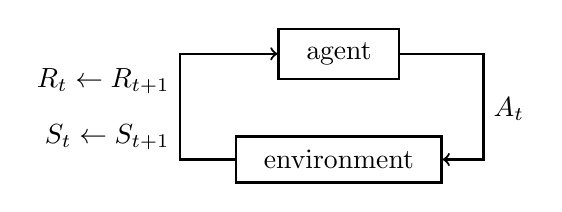
\begin{tikzpicture}
        \tikzset{
            rect/.style={draw, thick, rectangle, align=center, inner xsep=1em, inner ysep=.5em}
        }
        
        \node (origin) at (0, 0) {};
        \node (agent) [rect, right=2em of origin] {agent};
        \node (envir) [rect, below=2em of agent] {environment};
        % arrows
        \draw [thick, ->] (agent.east) -| node [right, yshift=-2em] {$A_t$} ++(3em, 0) |- (envir.east);
        \draw [thick, ->] (envir.west) -| ++(-2em, 0) |- node [left, yshift=-1em] {$R_t \leftarrow R_{t+1}$} node [left, yshift=-3em] {$S_t \leftarrow S_{t+1}$} (agent.west);
    \end{tikzpicture}
\end{figure}

\textit{State-Transition Probabilities (Alternative Forms)}

$p(s', r \mid s,a) \equiv \Pr \{ S_t = s', R_t = r \mid S_{t-1} = s, A_{t-1} = a \}$

$p(s' \mid s, a) = \Pr \{ S_t = s' \mid S_{t-1} = s, A_{t-1} = a \} = \sum_{r \in \mathcal R} p(s', r \mid s, a)$

$r(s, a) \equiv \mathbb E [R_t \mid S_{t-1} = s, A_{t-1} = a] = \sum_{r \in \mathcal R} r \sum_{s' \in \mathcal S} p(s', r \mid s, a)$

$r(s, a, s') \equiv \mathbb E [R_t \mid S_{t-1} = s, A_{t-1} = a, S_t = s'] = \sum_{r \in \mathcal R} r \frac{p(s', r \mid s, a)}{p(s' \mid s, a)}$

\dotfill

Markov property: future states of Markov process depend only on present state and not on past events.

Agent-envir interactions: episode $\to$ terminal state $\to$ reset

Goal of agent: maximize expected return, $G_t$

Episodic tasks: $G_t \equiv R_{t+1} + R_{t+2} + \cdots + R_T$

\vspace{-.5em}
\dotfill

\textit{Continuing Tasks (no terminal state)}

$G_t \equiv R_{t+1} + \gamma R_{t+2} + \gamma^2 R_{t+3} + \cdots + \gamma^{k-1} R_{t+k} + \cdots = \sum_{k=0}^\infty \gamma^k R_{t+k+1}$

$G_t = R_{t+1} + \gamma G_{t+1}$, \hfill $\sum_{k=0}^\infty \gamma^k = \frac{1}{1-\gamma},$ \hfill $\gamma \in [0, 1)$ is discount rate

$G_t \equiv \sum_{k=t+1}^T \gamma^{k-t-1} R_k$ \hfill $T = \infty$ or $\gamma = 1$ (but not both)

Notice that future rewards are discounted more.

$\quad \gamma = 0$: agent only cares about immediate reward (greedy).

$\quad \gamma \to 1$: future rewards contribute more.

\vspace{-.5em}
\dotfill

\textbf{Policies}

Law of total expectation: $\mathbb E[X] = \mathbb E[\mathbb E[X \mid Y]]$

$\quad$Partition formula: $\mathbb E[X] = \sum_i \mathbb E[X \mid A_i] P(A_i)$

Policy: mapping from states to probs of selecting each possible action.

$\quad \pi(a|s)= p(a \mid s) = \Pr \{ A_t = a \mid S_t = s \}$

Expectation of $R_{t+1}$ in terms of $\pi$ and $p$:

$\quad \mathbb E[R_{t+1} \mid S_t = s] = \sum_a \pi(a \mid S_t) \sum_{s', r} p(s', r \mid s, a) r$

\dotfill

\textbf{Value Functions}

Value fns give expected return $G_t$ when starting in state $s$ and following policy $\pi$ thereafter.

\textit{State-value fn:} $v_\pi(s) \equiv \mathbb E_\pi [G_t \mid S_t = s]$ \hfill $G_t = \sum_{k=0}^\infty \gamma^k R_{t+k+1}$

$\quad$Value of terminal state is always 0.

\textit{Action-value fn:} $q_\pi(s, a) \equiv \mathbb E_\pi [G_t \mid S_t = s, A_t = a]$

$\quad v_\pi$ in terms of $q_\pi$ and $\pi$: $v_\pi (s) = \sum_a \pi(a \mid S_t) q_\pi(s, a)$

$\quad q_\pi$ in terms of $v_\pi$ and $p$: $q_\pi(s, a) = \sum_{r, s'} p(s', r \mid s, a) [r + \gamma v_\pi(s')]$


\cleardoublepage


\textbf{Bellman Equations}

$v_\pi(s) = \sum_a \pi(a \mid s) \sum_{s', r} p(s', r \mid s, a) [r + \gamma v_\pi(s')]$

$q_\pi(s,a) = \sum_{s', r} p(s',r \mid s,a) \left[ r + \gamma \sum_{a'} \pi(a' \mid s') q(s', a') \right]$

\textit{Optimal value fns:} $\pi_1 \geq \pi_2 \iff v_{\pi_1}(s) \geq v_{\pi_2}(s), \quad \forall s \in \mathcal S$

$\quad v_*(s) = \max_\pi v_{\pi}(s) = \max_a \sum_{s', r} p(s', r \mid s, a) [r + \gamma v_*(s')], \quad \forall s \in \mathcal S$

$\quad q_*(s, a) = \max_{\pi} q_\pi(s,a) = \sum_{s', r} p(s', r \mid s, a) [ r + \gamma \max_{a'} q_*(s', a')]$

$\quad \quad \forall s \in \mathcal S, \forall a \in \mathcal A$

\vspace{-.5em}
\dotfill

\textbf{Policy Evaluation}

$\pi_* = \argmax_a \sum_{s', r} p(s',r \mid s, a)[r + \gamma v_*(s')]$

\begin{mydef}{Iterative Policy Evaluation}{}
    Input $\pi$, the policy to be evaluated \\
    $\vec V \leftarrow \vec 0, \vec V' \leftarrow \vec 0$ \\
    loop: \\
        \hspace*{2em} $\Delta \leftarrow 0$ \\
        \hspace*{2em} loop for each $s \in \mathcal S$: \\
            \hspace*{4em}$V'(s) \leftarrow \sum_a \pi(a \mid s) \sum_{s', r} p(s', r \mid s, a) [r + \gamma V(s')]$ \\
            \hspace*{4em}$\Delta \leftarrow \max(\Delta, |V'(s) - V(s)|)$ \\
        \hspace*{2em}$V \leftarrow V'$ \\
    until $\Delta < \theta$ (small positive number) \\
    return $V \approx v_\pi$
\end{mydef}

\textit{Policy improvement thm:} $q_\pi(s, \pi'(s)) \geq v_\pi(s), \quad \forall s \in \mathcal S$

$\pi'(s) \equiv \argmax_a q_\pi(s,a) = \argmax_a \sum_{s', r} p(s',r \mid s,a) [r + \gamma v_\pi(s')]$

\begin{mydef}{Policy Iteration}{}
    1. Initialization \\
    $V(s) \in \mathbb R$ and $\pi(s) \in \mathcal A(s)$ arbitrarily $\forall s \in \mathcal S$ \\
    
    2. Policy Evaluation \\
    Loop: \\
        \hspace*{2em}$\Delta \leftarrow 0$ \\
        \hspace*{2em}Loop for each $s \in \mathcal S:$ \\
            \hspace*{4em}$v \leftarrow V(s)$ \\
            \hspace*{4em}$V(s) \leftarrow \sum_{s', r} p(s', r \mid s, \pi(s)) [r + \gamma V(s')]$ \\
            \hspace*{4em}$\Delta \leftarrow \max(\Delta, |v - V(s)|)$ \\
    
    3. Policy Improvement \\
    \textit{policy-stable} $\leftarrow$ true \\
    For each $s \in \mathcal S$: \\
        \hspace*{2em}\textit{old-action} $\leftarrow \pi(s)$ \\
        \hspace*{2em}$\pi(s) \leftarrow \argmax_a \sum_{s', r} p(s', r \mid s,a)[r + \gamma V(s')]$ \\
        \hspace*{2em}If \textit{old-action} $\neq \pi(s)$, then \textit{policy-stable} $\leftarrow$ false \\
    If \textit{policy-stable}, then stop and return $V \approx v_*$ and $\pi \approx \pi_*$; else go to 2.
\end{mydef}




\end{document}
